\documentclass[conference]{IEEEtran}

\usepackage[latin1]{inputenc}	% for Latin languages
\usepackage[T1]{fontenc}	% for ISO and UTF characters
\usepackage[english]{babel}	% for multilingual support
\usepackage{graphicx}
\usepackage{subfig}

\newcommand{\fig}[4][htbp]{
  \begin{figure}[#1] {\centering\scalebox{#2}{\includegraphics{fig/#3}}\par}
    \caption{#4\label{#3}}
  \end{figure}
}

\newcommand{\epos}{\textsc{Epos}}

\begin{document}

\title{C-MAC and ADHOP: towards a cross-layer integration for WSNs}

\author{Names\\
  \\
  Software/Hardware Integration Lab\\
  Federal University of Santa Catarina\\
  PO Box 476, 88040-900 - Florian�polis, SC, Brazil \\
  \{names\}@lisha.ufsc.br
}

\maketitle

\begin{abstract}
In Wireless Sensor Networks (WSNs), Medium Access Control (MAC) protocols have the most accurate information regarding links between sensor nodes,
such as Received Signal Strength Indicator (RSSI) and Link Quality Indicator (LQI).
Nevertheless, traditional communication protocol stacks do not receive the direct benefits of this information which could be used to assist decisions on upper layers.
Furthermore, MAC protocols can also provide resource information like residual energy and memory concerning neighboring nodes, by attaching this information into data packets.
Such knowledge may be used, for example, by routing protocols in order to enhance the discovery and maintenance of network routes.
In this paper, we present the integration between the Configurable MAC (C-MAC) and Ant-based Dynamic Hop Optimization Protocol (ADHOP), a routing scheme for dynamic WSNs.
In our proposal, both C-MAC and ADHOP share a structure in which C-MAC provides several information which can be used as routing heuristics by ADHOP.
We have evaluated our integration by comparing the performance of ADHOP with and without the information provided by C-MAC.
The experimental results presented in the paper corroborate that our proposal achieves a higher data delivery ratio, lower routing overhead, and better results in balancing energy.
% insert our results numbers here when we finally get them.
\end{abstract}

\section{Introduction}
\label{sec:intro}

The rest of this paper is organized as follows.
Section~\ref{sec:cmac_adhop} describes both protocols used in this work: C-MAC and ADHOP.
Section~\ref{sec:integration} describes the integration between the protocols.
Section~\ref{sec:results} presents an evaluation of our proposal, followed by our conclusions in Section~\ref{sec:conclusions}.

\section{?}
\label{sec:cmac_adhop}
\subsection{C-MAC}
\label{subsec:cmac}
C-MAC is a highly configurable MAC protocol for WSNs realized as a framework of
medium access control strategies that can be combined to produce
application-specific protocols~\cite{steiner:2010}. It enables application
programmers to configure several communication parameters (e.g.  synchronization,
contention, error detection, acknowledgment, packing, etc) to adjust the protocol
to the specific needs of their applications. The framework was implemented in C++ 
using static metaprogramming techniques (e.g. templates, inline functions, and 
inline assembly), thus ensuring that configurability does not come at expense of 
performance or code size. The main C-MAC configuration points include:

\textbf{Physical layer configuration:} These are the configuration points defined
by the underlying transceiver (e.g. frequency, transmit power, date rate).

\textbf{Synchronization and organization:} Provides mechanisms to send or receive
synchronization data to organize the network and synchronize the nodes duty
cycle.

\textbf{Collision-avoidance mechanism:} Defines the contention mechanisms used to
avoid collisions. May be comprised of a carrier sense algorithm (e.g. CSMA-CA),
the exchange of contention packets (\emph{Request to Send} and \emph{Clear to
Send}), or a combination of both.

\textbf{Acknowledgment mechanism:} The exchange of \emph{ack} packets to
determine if the transmission was successful, including preamble acknowledgements.

\textbf{Error handling and security:} Determine which mechanisms will be used to
ensure the consistency of data (e.g. CRC check) and the data security.

\subsection{ADHOP}
\label{subsec:adhop}

ADHOP is a self-configuring and multi-hop reactive routing protocol that aims to provide routing for dynamic WSNs.
It aims at dynamic network topologies in order to avoid congestion and link failures, and improve the discovery and maintenance of routes.
It is inspired on the HOPNET algorithm which uses Ant Colony Optimization (ACO) \cite{Dorigo:2005, Dorigo:2006} and Zone Routing Protocol (ZRP) \cite{Haas:1997} to handle important problems in Mobile Ad hoc NETworks (MANETs) \cite{Wang:2009}.

The idea behind routing protocols based on ACO is to apply the behaviour of ants in the network to discover and maintain the best routes among the nodes.
These protocols can thereby maintain the routing table efficiently updated due to the proportionate dynamism of ants to detect changes in the network topology by pheromone.
ADHOP abstracts the concept of zones and focus on the next hop that the ant has to perform.

Each node in ADHOP can store an amount of pheromone between itself and any other node in the network, i.e., all routing decisions are made locally, without needing to know the entire network to route the data.
In order to make routing decisions properly, the ants are responsible for dissipating the knowledge of the network and to teach to nodes the best route to be taken at that instant.
The nodes do not need to be concerned to discover and maintain entire routes to particular nodes.
They just need to direct the data to the next hop toward the destination node through a local decision.
The routes are not predetermined and the hops are chosen dynamically at each step toward the destination.
Hence, ADHOP can adapt to topology changes transparently, as in situations shown in Figure \ref{dynamic}.

\begin{figure*}[htb]
\centering
\begin{tabular}{c c c}
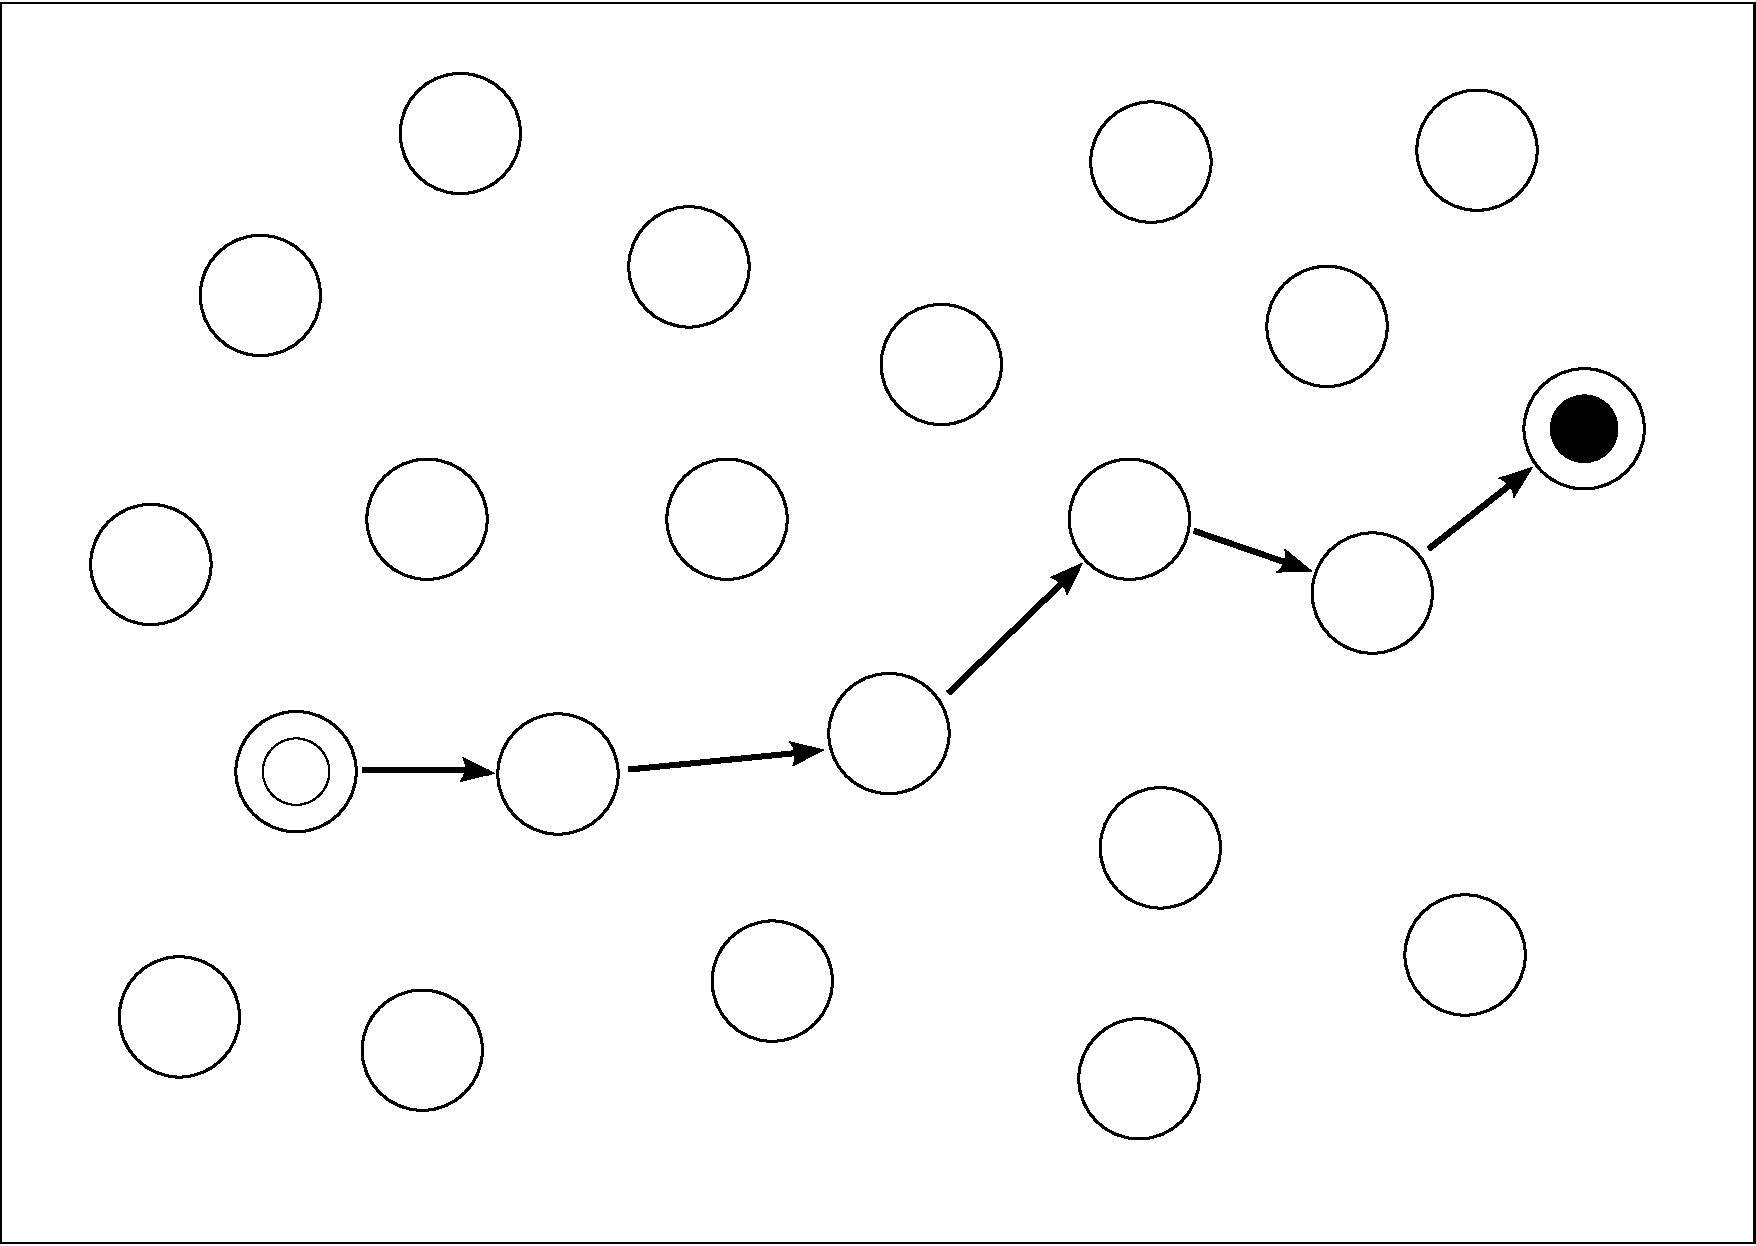
\includegraphics[width=130pt]{fig/dynamic_1.pdf} &
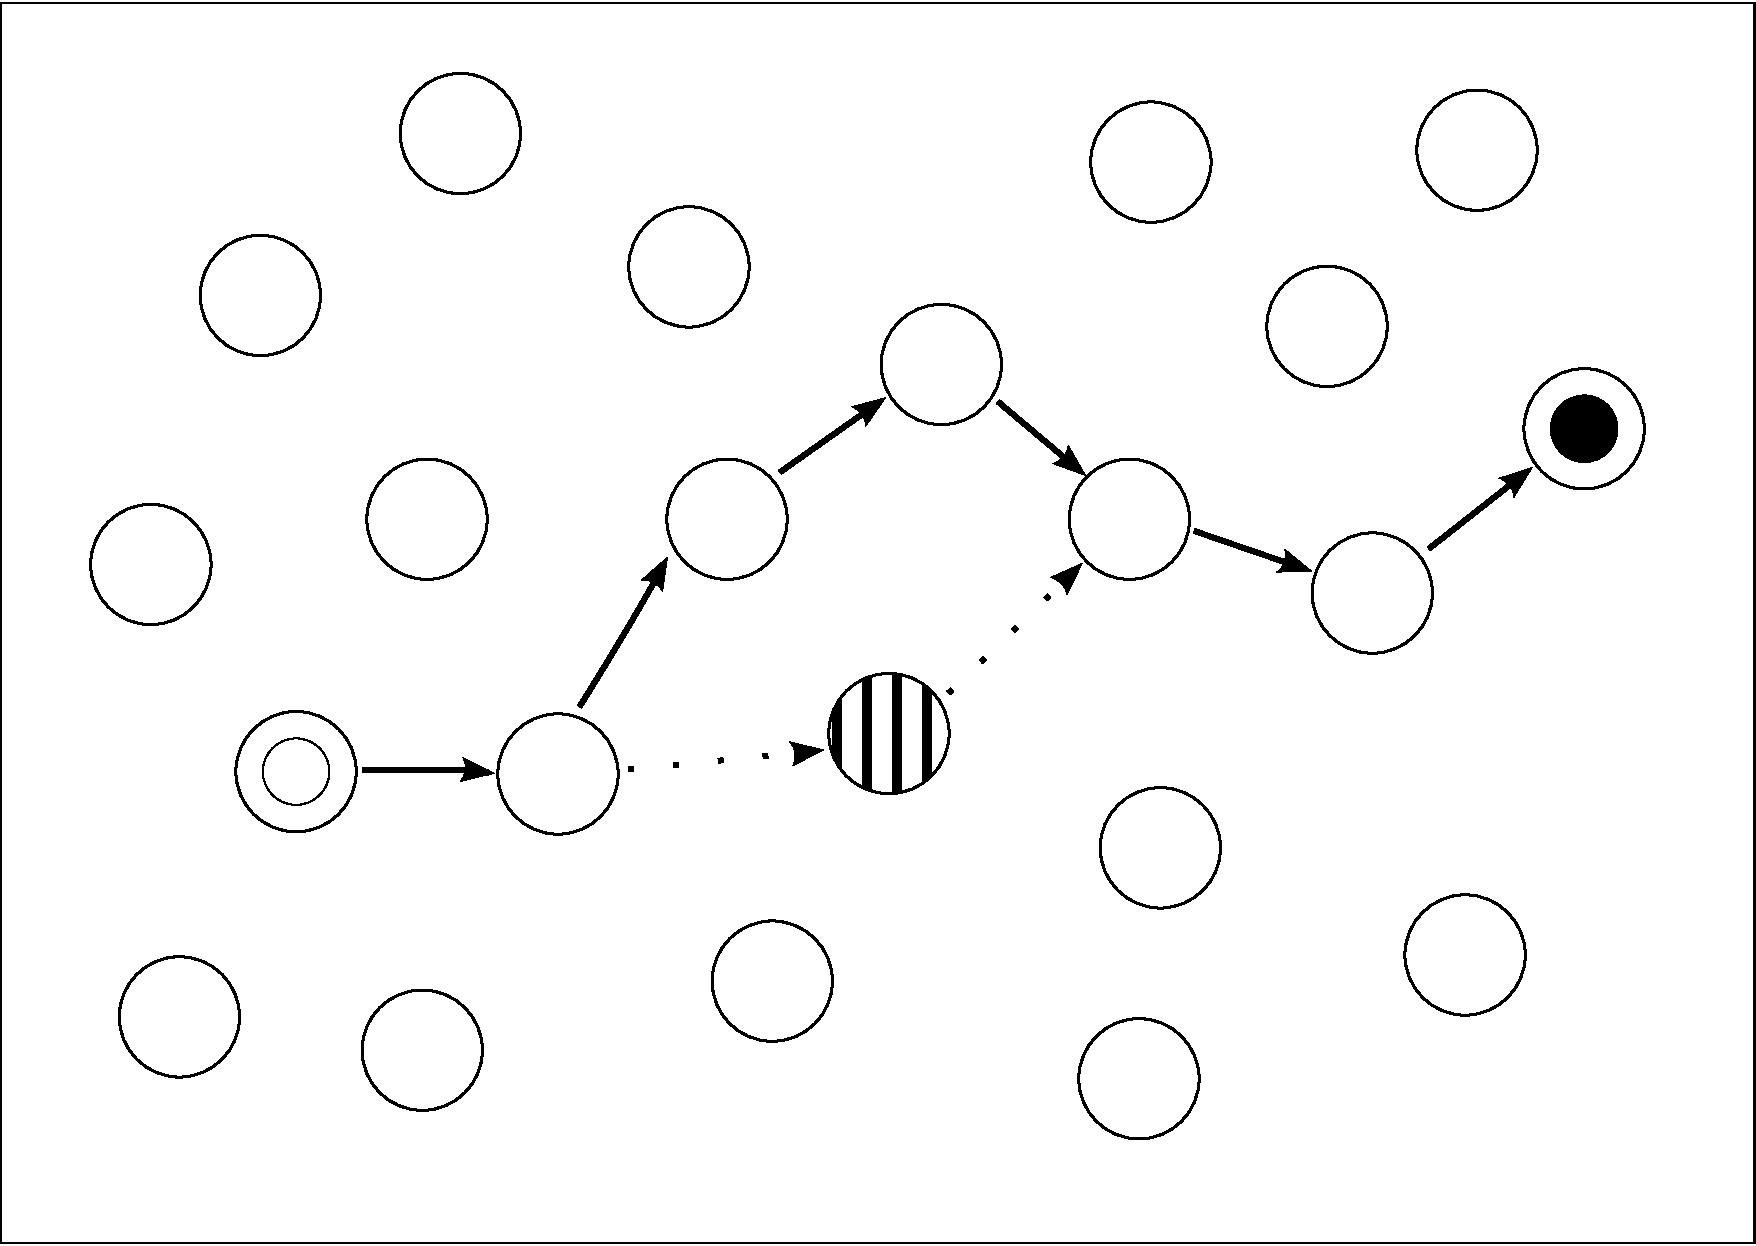
\includegraphics[width=130pt]{fig/dynamic_2.pdf} &
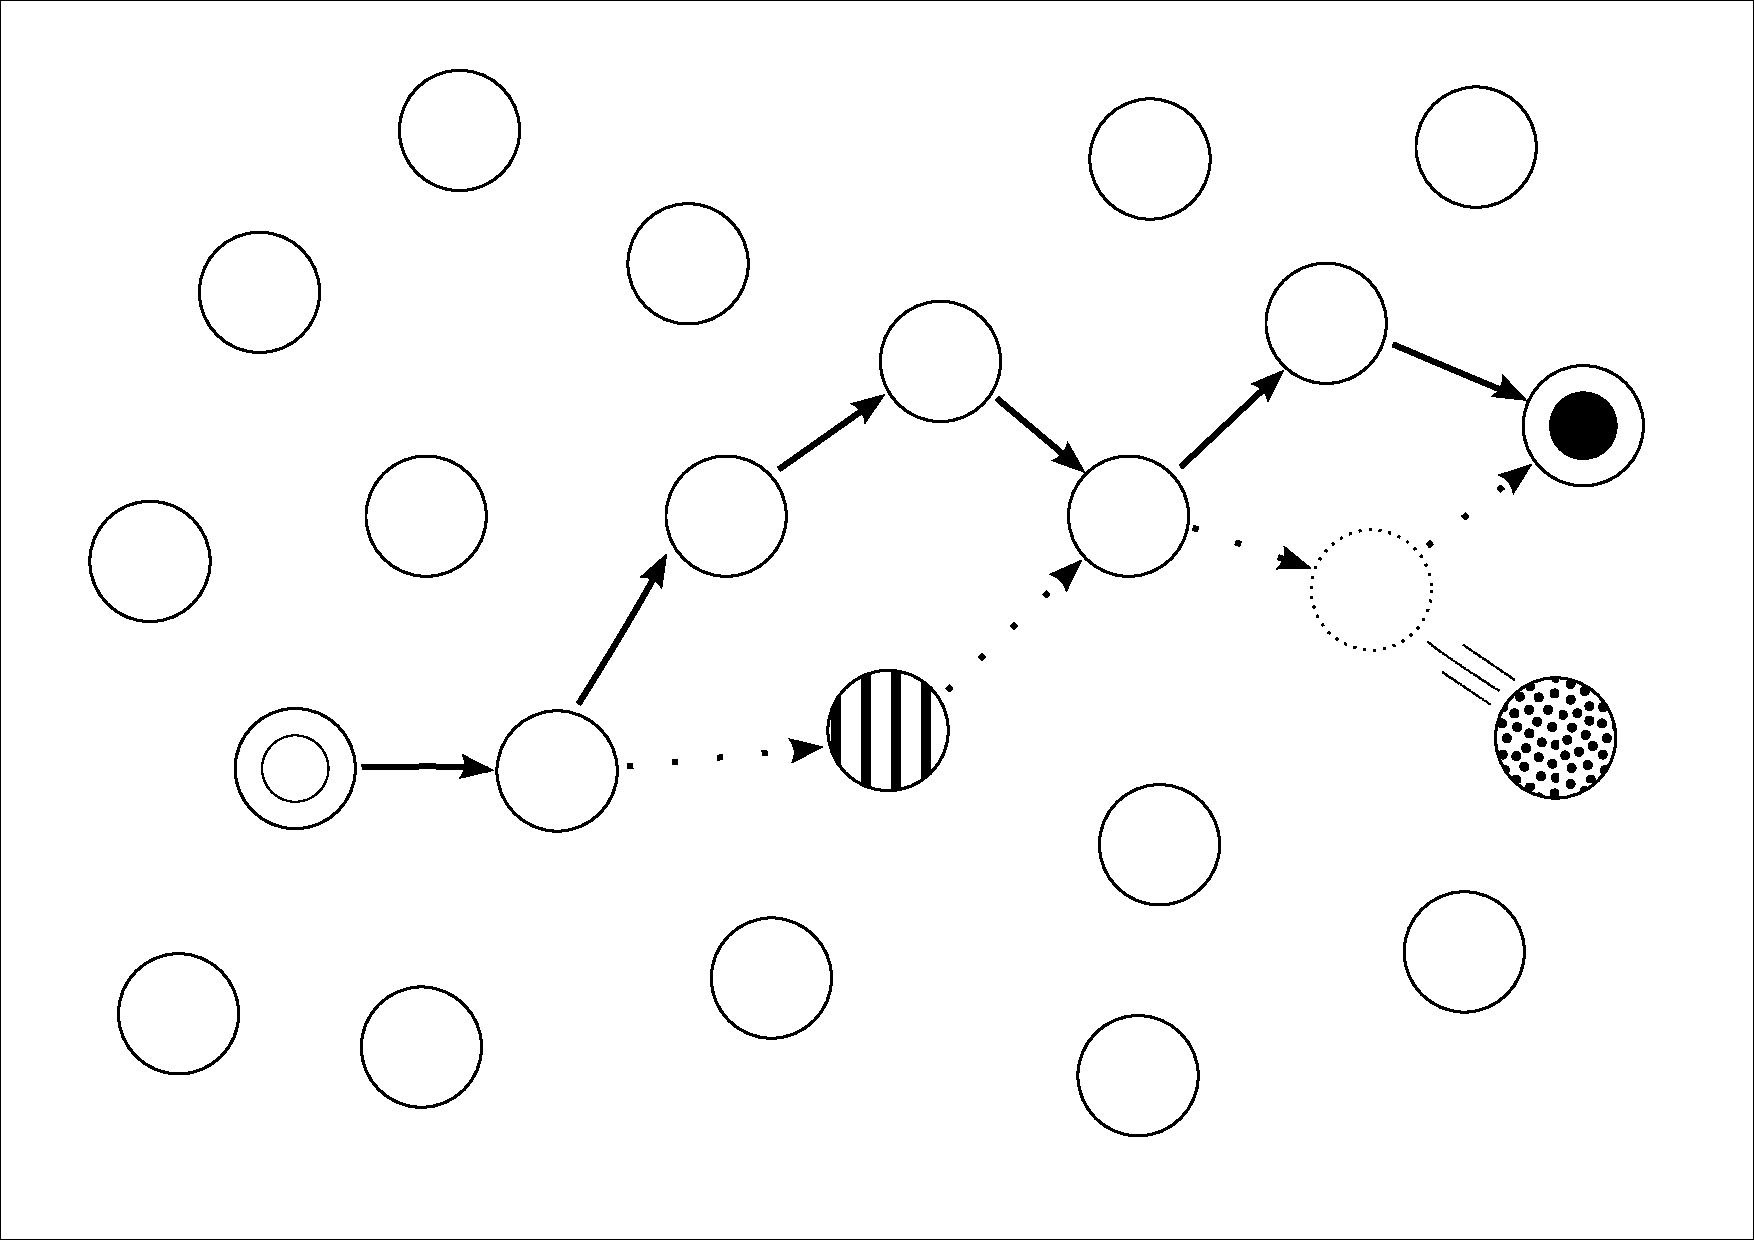
\includegraphics[width=130pt]{fig/dynamic_3.pdf} \\
\multicolumn{3}{c}{ 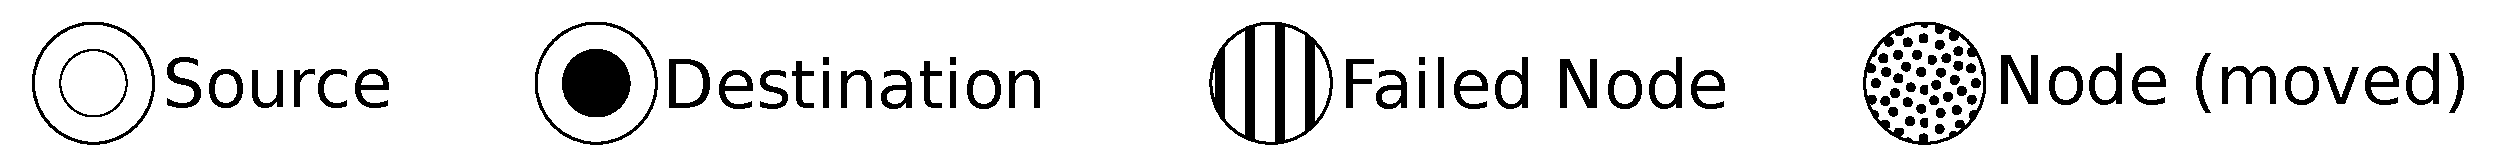
\includegraphics[width=180pt]{fig/dynamic_subtitle.pdf} } \\
(a) & (b) & (c) \\
\end{tabular}
\caption{Dynamic Hops.}
\label{dynamic}
\end{figure*}

In Figure \ref{dynamic} (a), from the source to a particular destination, the ADHOP algorithm define the best route by pheromone.
In Figure \ref{dynamic} (b), one of the nodes along the route fail, and an alternative route is defined.
The same happens when a node moves from the route, as shown in Figure \ref{dynamic} (c).
In order to maintain updated routes, the pheromone between nodes is evaporated periodically.
If part of a route is no longer used, then nodes can also leave the routes due to pheromone evaporation.

Differently from HOPNET, which uses two routing tables, ADHOP uses a unique routing table structure similar to HOPNET Intrazone Routing Table (IntraRT).
Its operations are simple and fast, and routes beyond the zones do not need to be stored entirely like the other HOPNET routing table.
The nodes can thereby use simple operations to deal with dynamic changes along the routes.
In order to accomplish these routing operations, a new collection of ants is presented: \emph{internal transport ant} (ITA) and \emph{exploratory transport ant} (ETA).
Although each ant category has a different function, they share a common data structure.
Figure \ref{adhop_protocol} shows the ant data structure of ADHOP.

\begin{figure}[htb]
\centering
\begin{tabular}{c}
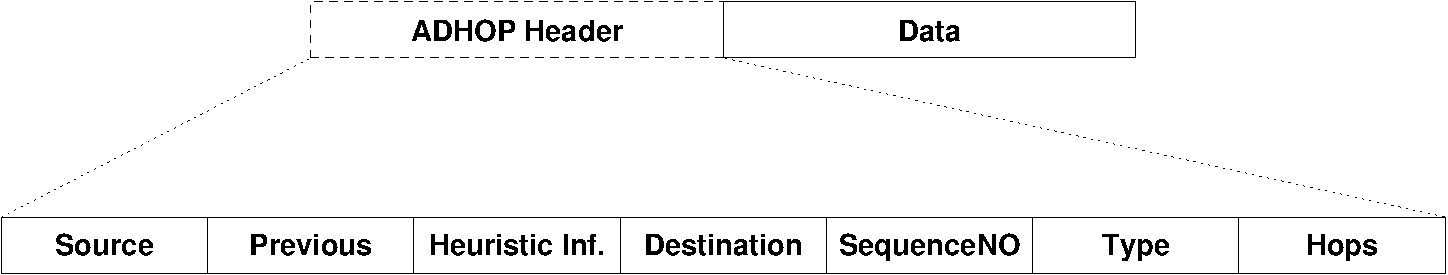
\includegraphics[width=220pt]{fig/adhop_protocol.pdf}
\end{tabular}
\caption{ADHOP Ant Structure.}
\label{adhop_protocol}
\end{figure}

The data structure includes address fields as \emph{Source} and \emph{Destination}.
The \emph{Previous} field is responsible for storing the address of the previous node.
The \emph{SequenceNO} field is used for control.
The \emph{Type} field indicates the ant category, and the \emph{Hops} field indicates the number of hops which the ant has done.
The \emph{Heuristic Inf.} field is responsible for storing the necessary heuristic information to calculate the evaporation and the pheromone deposit ratio.
These ants help to reduce the complexity to offer better tactics to diffuse and verify pheromone among the nodes, reinforcing the links between neighbors to maintain the best routes according to the heuristic information.
In addition, both ITA and ETA perform data delivery while they deposit pheromone on the route which they travel.

Figure \ref{adhop_data_tx} depicts the sequence diagram for data transmission in ADHOP.
In ADHOP, the data packet is sent along with the ant to ensure that sudden changes in the network do not interfere with the transportation of the data towards the destination.
The data packet may thereby be dynamically redirected to a safer route, as depicted in Figure \ref{dynamic}.

\begin{figure}[htb]
\centering
\begin{tabular}{c}
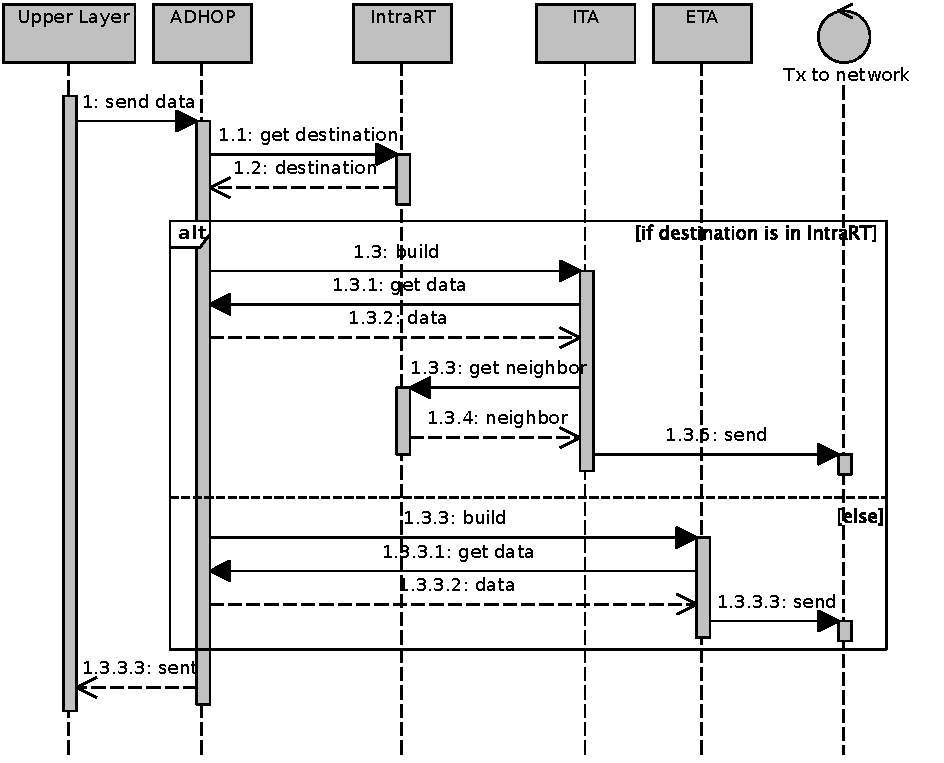
\includegraphics[width=220pt]{fig/adhop_data_tx.pdf}
\end{tabular}
\caption{ADHOP - Data Transmission.}
\label{adhop_data_tx}
\end{figure}

ETAs are responsible for discovering routes to unknown nodes.
These ants travel through the network to discover the destination node.
At the destination, the ETA delivers the data packet and returns to the source node.
On the way back, the ant just sets the pheromone trail in order to add it to the zone.

ITAs are responsible for delivering data packets.
When a source node discovers a new route to certain destination by ETA, the following data packet transmissions are performed by ITAs until the pheromone amount on the route evaporates entirely.
Nevertheless, at any time, if any route to any destination breaks, any node on the route can use an ETA to recover it or discover a new path.
It allows us to deal with dynamic network topologies and avoid as much as possible broken routes.

ADHOP uses the following equations for deposit and evaporation of pheromone.
Each ant selects a node $v_{j}$ as the next hop from the current node $v_{i}$.
Actually, node $v_{j}$ has the largest amount of pheromone among neighboring towards the destination node $v_{d}$.
At the node $v_{j}$, the ant updates the pheromone $\tau _{i,s}$ on the entry $\left ( v_{i},v_{s} \right )$ in routing table, where $v_{s}$ is the source node, as follows \cite{Dorigo:2006}:
\begin{equation} \tau _{i,s} = \left ( 1 - \varphi \right ) \cdot \tau _{i,s} + \varphi \cdot \tau _{0} \label{adhop_pheromone_increasing} \end{equation}
where $\tau _{0}$ is the initial value of pheromone, and $\varphi \in \left [ 0,1  \right )$ is the pheromone decay coefficient which is calculated from the heuristic information (Figure \ref{adhop_protocol}) of the node $v_{i}$.

The equation (\ref{adhop_pheromone_increasing}) allows us to diversify the search process by increasing or decreasing the pheromone amount in the routes while allowing other ants to achieve different routes.
It also helps to increase the effect of dynamic hops, allowing us to deal with dynamic network topologies, avoiding the possible broken routes, and adapting to the needs of the network through the heuristic information.

The evaporation occurs periodically to all nodes in the network, using the following equation:
\begin{equation} \tau _{i,j} = \left ( 1 - \rho \right ) \cdot \tau _{i,j} , \quad \forall i \in N, \quad \forall j \in Z \label{evaporation} \end{equation}
where $\rho \in \left [ 0,1  \right )$ is the evaporation ratio, $N$ is the set of neighbor nodes, and $Z$ is the set of nodes which, together with neighbor nodes, define entries $\left ( v_{i},v_{j} \right )$ in routing table.

ADHOP also aims to abstract problems in the network and handle topology changes only through pheromone to avoid additional overhead in the network as well as possible congestion.
Congestion usually causes packet loss, queueing delay, and consequently less pheromone deposit.
Since our routing table structure maintains pheromone information between nodes in the zone, it does not need to be updated at each change in network topology.
These changes in topology are observed unwittingly by ants.
Thereupon, control packets to notify or fix routing errors are unnecessary.
It allows us to handle congestion the way that complex operations in the network can be avoided.

\section{Integration}
\label{sec:integration}

\section{Experimental results}
\label{sec:results}

\section{Conclusion}
\label{sec:conclusions}

\bibliographystyle{IEEEtran}
\bibliography{references}

\end{document}
